\begin{frame}
    \Huge
    \begin{center}
        Simulasi dan Pembuatan Sub-Sistem
    \end{center}
\end{frame}


\begin{frame}
    \frametitle{Pengambilan Data Lidar}
    
    Data yang dihasilkan oleh Lidar memiliki format *.bin yang tidak dapat dibaca secara langsung dan perlu diproses ke dalam bentuk kumpulan set posisi point cloud (*.pcd). Kumpulan set ini dapat ditampilkan dalam plot 3D seperti Gambar berikut

    \begin{figure}
        \centering
        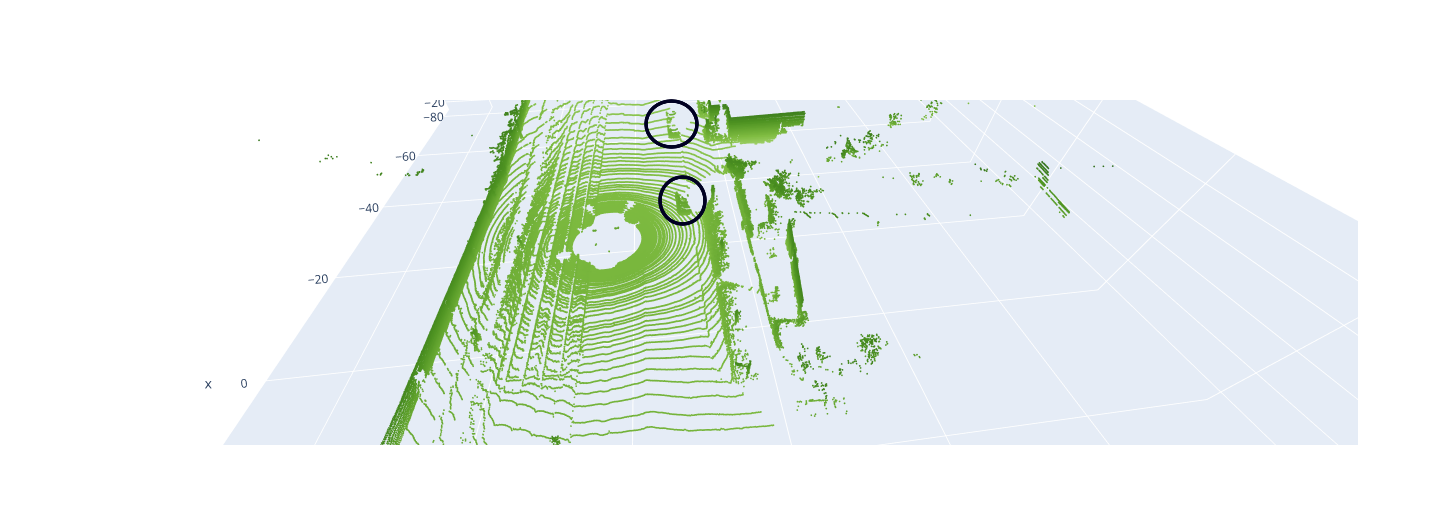
\includegraphics[width=\textwidth]{lidar-raw.png}
        \label{fig: lidar-plot3d-raw}
    \end{figure}
\end{frame}


\begin{frame}[allowframebreaks]
    \lstset{
  caption=Program konversi data *.bin Lidar menjadi \textit{list of point cloud set}, 
  label={lst: bin2pcd},
  basicstyle=\footnotesize, frame=tb,
  language=python
}
\begin{lstlisting}
def bin2pcd(binFileName):
    size_float = 4
    list_pcd = []
    with open(binFileName, "rb") as f:
        byte = f.read(size_float * 4)
        while byte:
            x, y, z, intensity = struct.unpack("ffff", byte)
            list_pcd.append([x, y, z])
            byte = f.read(size_float * 4)
    np_pcd = np.asarray(list_pcd)
    pcd = o3d.geometry.PointCloud()
    pcd.points = o3d.utility.Vector3dVector(np_pcd)
    return pcd
\end{lstlisting}
\end{frame}


\begin{frame}
    \frametitle{Lidar Clustering}
    Lidar Clustering adalah metode untuk mengelompokkan point cloud yang dihasilkan oleh lidar ke dalam cluster berdasarkan jarak eucledian antara satu titik dengan titik lainnya. Terdapat beberapa langkah yang perlu dilakukan untuk mengimplementasikan metode ini, yakni:

    \begin{itemize}
        \item Voxel Grid Processing \\
        \item Terrain Removal \\
        \item Eucledian Clustering \\
        \item Asosiasi
    \end{itemize}
\end{frame}


\begin{frame}
    \frametitle{Voxel Grid Processing}

    Data point cloud ini memiliki jumlah yang sangat banyak ($3 \times 10^5$ hingga $2 \times 10^6$ titik) sehingga akan sangat membebani algoritma clustering. Untuk mengurangi jumlah data yang digunakan, maka dapat dilakukan reduksi data point cloud dengan menggunakan metode Voxel Grid \cite{open3d_2018}. Keluaran dari metode Voxel Grid ini memiliki jumlah data yang lebih sedikit, namun tidak mengurangi kemampuan deteksi secara signifikan \cite{open3d_2018}.
    \begin{figure}
        \centering
        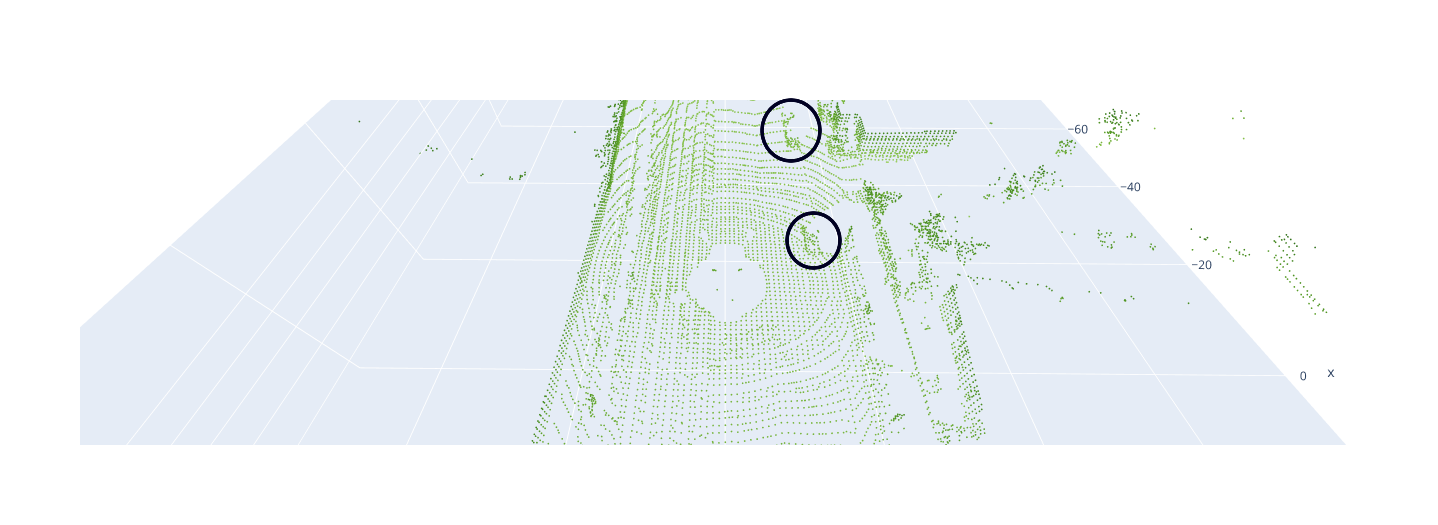
\includegraphics[width=\textwidth]{lidar-voxelize.png}
    \end{figure}
\end{frame}


\begin{frame}[allowframebreaks]
    \lstset{
  caption=Program voxel grid, 
  label={lst: voxelgrid},
  basicstyle=\footnotesize, frame=tb,
  language=python
}
\begin{lstlisting}
downpcd = pcd.voxel_down_sample(voxel_size=0.5)
o3d.visualization.draw_geometries([downpcd])
cloud_xyz = np.asarray(downpcd.points) # get xyz points
\end{lstlisting}

    Pada library Open3D telah terdapat function untuk melakukan operasi voxel grid yang dapat langsung digunakan. 
\end{frame}


\begin{frame}
    \frametitle{Terrain Removal}

    Setelah data point cloud direduksi menggunakan Voxel Grid, kita dapat menghilangkan bidang jalan dengan mencari bidang datar di sekitar lokasi $z$ minimal.Metode ini hanya efektif bila jalan berupa bidang datar.
    \begin{figure}
        \centering
        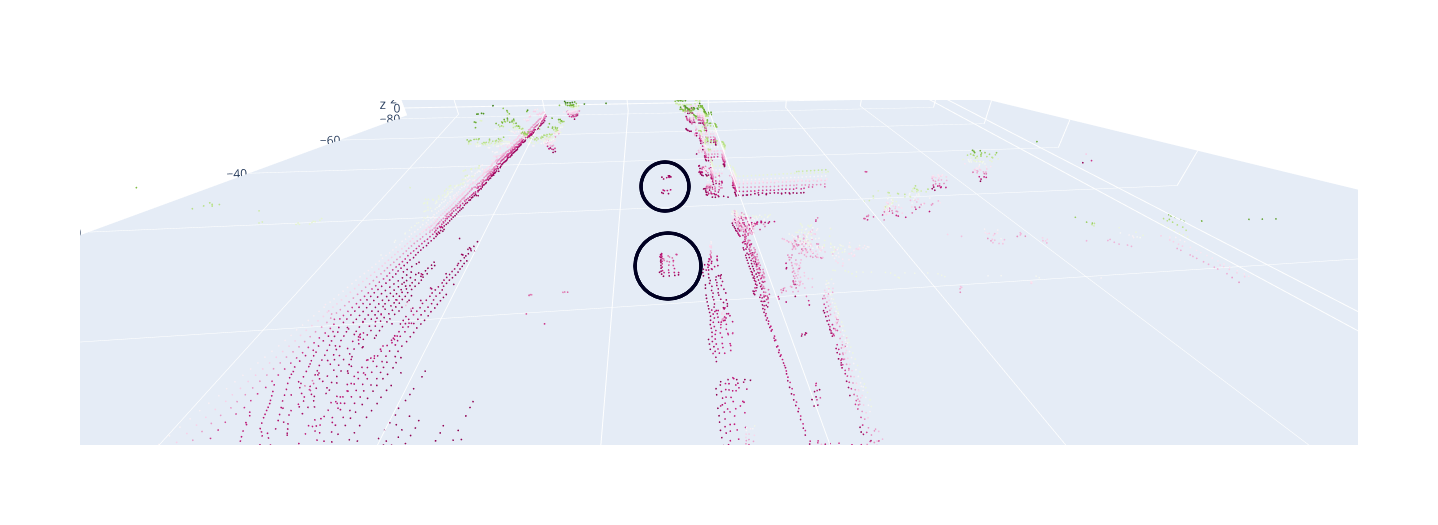
\includegraphics[width=\textwidth]{lidar-remove-floor.png}
    \end{figure}
\end{frame}


\begin{frame}[allowframebreaks]
    \lstset{
  caption=Program menghilangkan bidang jalan, 
  label={lst: removefloor},
  basicstyle=\footnotesize, frame=tb,
  language=python
}
\begin{lstlisting}
def filter_ground(cloud):
  # range antara min and max di sb-z dgn 0.1 step
  bin_range = np.arange(cloud[:,2].min(),cloud[:,2].max(), 0.1)
  # find distribution of points in z-axis
  counts, bins = np.histogram(cloud[:,2], bins = bin_range)
  # find for which z there is maximum points
  max_z = np.where(counts == max(counts))[0][0]
  # check max_z + 2 tidak overflow
  if max_z + 2 <= len(bins):
      ground_z = np.round(bins[max_z + 2], 2)
  else:
      ground_z = np.round(bins[-1], 2)
  # remove ground points
  objects_cloud = cloud[(cloud[:,2]>ground_z)]
  
  return objects_cloud, ground_z
\end{lstlisting}
\end{frame}


\begin{frame}
    \frametitle{Eucledian Clustering}

    Pada langkah ini setiap titik diiterasi untuk menghitung apakah titik ini termasuk kedalam cluster yang sama atau cluster yang berbeda.
    \begin{figure}
        \centering
        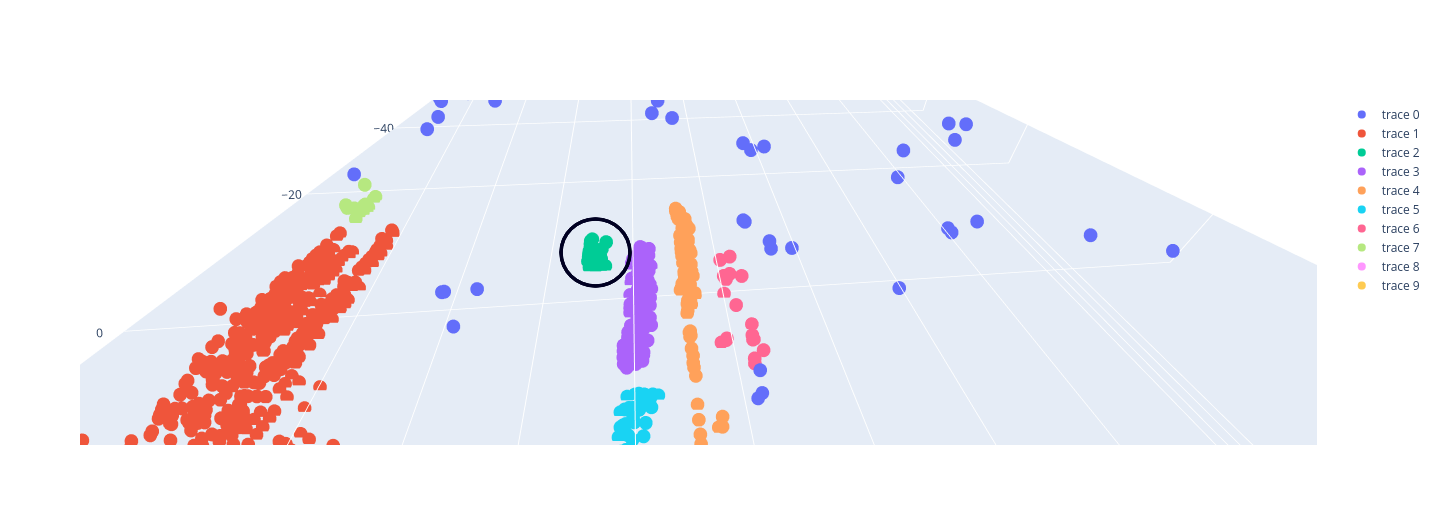
\includegraphics[width=\textwidth]{lidar-clustering.png}
    \end{figure}
\end{frame}


\begin{frame}
    \frametitle{Asosiasi}

    Langkah terakhir adalah melakukan deteksi dan penentuan bounding box pada cluster yang dianggap sebagai mobil. Langkah ini masih belum selesai dikerjakan
\end{frame}


\begin{frame}
    \frametitle{Multi-Object Tracking}

    Program Multi-Object Tracking ini terbagi kedalam dua bagian besar:
    \begin{enumerate}
        \item Filtering
        \item Track Selection
    \end{enumerate}
\end{frame}


\begin{frame}
    \frametitle{Filtering}

    Pada ujicoba ini, filtering masih menggunakan filter kalman dasar karena terdapat error pada program filtering dengan Extended Kalman Filter yang diusulkan. Model yang digunakan pada kalman filter dasar ini tidak mempertimbangkan heading kendaraan karena heading kendaraan menyebabkan nonlinearitas pada sistem yang menyebabkan kalman filter dasar tidak dapat digunakan.
\end{frame}


\begin{frame}
    \frametitle{Track Selection}

    \begin{itemize}
        \item Track merupakan object yang digunakan untuk melakukan tracking pada halangan yang terdeteksi. 
        \item Setiap track memiliki posisi awal yang diinisialisasi berdasar hasil deteksi halangan pertama. 
        \item Pada deteksi ke-2 dan seterusnya (proses update), akan dilakukan prediksi pergerakan objek menggunakan filter Kalman. 
        \item Halangan yang posisinya paling dekat ke hasil prediksi akan dianggap sebagai halangan yang sama. 
        \item Apabila halangan tidak terdeteksi, Track akan terus melakukan prediksi hingga N langkah ke depan sebelum menghapus objek Track.
    \end{itemize}
\end{frame}


\begin{frame}
    \centering
    \animategraphics[loop, autoplay, width=.5\textwidth]{24}{animasi-tracking/image}{15}{130}
\end{frame}